%%%%%%%%%%%%%%%%%%%%%%%%%%%%%%%%%%%%%%%%%%%%%%%%%%%%%%%%%%%
% --------------------------------------------------------
%  ____  _           
% |  _ \| |__   ___  
% | |_) | '_ \ / _ \ 
% |  _ <| | | | (_) |
% |_| \_\_| |_|\___/ 
%
% LaTeX2e Template
% Version 3.0.0 (24/02/2026)
%
% Author: 
% Guillermo Jimenez (memo.notess1@gmail.com)
% 
% Contributor:
% Eduardo Gracidas (eduardo.gracidas29@gmail.com)
%
% License:
% Creative Commons CC BY 4.0
% --------------------------------------------------------
%%%%%%%%%%%%%%%%%%%%%%%%%%%%%%%%%%%%%%%%%%%%%%%%%%%%%%%%%%%
% --------------------------------------------------------
% Find the latest version on GitHub:
% https://github.com/MemoJimenez/Rho-class
% --------------------------------------------------------
%%%%%%%%%%%%%%%%%%%%%%%%%%%%%%%%%%%%%%%%%%%%%%%%%%%%%%%%%%%

\documentclass[9pt,a4paper,twocolumn,twoside]{rho-class/rho}
\usepackage[english]{babel}

%% Spanish babel recomendation
% \usepackage[spanish,es-nodecimaldot,es-noindentfirst]{babel}

% Using \doublespacing in the preamble 
% changes the text to double-line spacing
\onehalfspacing

%----------------------------------------------------------
% Title
%----------------------------------------------------------

\doctype{Systematic Review}
\title{State-of-the-Art Research Survey in Deep Learning}

%----------------------------------------------------------
% Authors, Affiliations and dates
%----------------------------------------------------------

\author[{\textasteriskcentered}1]{Kenji Omar Ramírez}
\author[{\textdagger}1]{Alejandro Elí Acosta Flores}
\author[{\textdagger}1]{Gabriel Emmanuel Monroy Romo}
\author[{\textdagger}1]{María de los Angeles Rabelero Campos}

%----------------------------------------------------------

\affil[1]{Master in Applied Artificial Intelligence, Instituto Tecnologico y de Estudios Superiores de Monterrey}

%----------------------------------------------------------

\dates{Received: 23 Mar 2026}

%----------------------------------------------------------
% Corresponding author-, Document- information
%----------------------------------------------------------

\corres{\textsuperscript{\textasteriskcentered}Corresponding authors: \href{mailto:A01796851@tec.mx}{A01796851@tec.mx} (K. O. Ramírez), \href{mailto:A01100001@tec.mx}{A01100001@tec.mx} (A. E. Acosta), \href{mailto:A01797342@tec.mx}{A01797342@tec.mx} (G. E. Monroy), \href{mailto:A01796851@tec.mx}{A01796851@tec.mx} (M. A. Rabelero)}
\corres{\textsuperscript{\textdagger}These authors contributed equally to this work.}

%----------------------------------------------------------

%\docinfo{This document class was prepared on Overleaf and compiled with pdf\LaTeX{}. No errors were found during the compilation process. Rho-class supports external editors, though additional setup may be required.} 

%----------------------------------------------------------

\journalname{Artificial Intelligence Review}
\journal{Springer Nature 2026}
\theday{\today}
\vol{59}
\issue{4}

%----------------------------------------------------------
% Abstract and Keywords
%----------------------------------------------------------

\begin{abstract}
    The rapid evolution of Deep Learning, particularly through diffusion models and generative architectures, has transformed the audiovisual landscape. This paper surveys the current state of image and video generation, focusing on their integration into artistic workflows for cinema and video games. We analyze the technical acceleration provided by these models—such as Text-to-3D and physics-grounded motion—while critically addressing the ethical crises they precipitate. Central to this discussion are the challenges of copyright, regional stereotypes, and the rise of deepfakes. By reviewing recent literature (2024-2026), we propose a framework that balances technical efficiency with ethical responsibility and human-centric authorship.
\end{abstract}

%----------------------------------------------------------

\keywords{AI ethics, Misinformation Risks, Intellectual Property (IP) Concerns, Responsible AI, Copyright compliance}

%----------------------------------------------------------

\begin{document}

    \maketitle
    \thispagestyle{firststyle}

%----------------------------------------------------------

\section{Introduction}

    \rhostart{I}n the current technological epoch,Artificial Intelligence (AI) has transcended its role as a mere automation tool to become a "collaborative agent". In the audiovisual and video game industries, generative models do not merely replace the artist but establish an interactive dialogue that optimizes creative phases previously burdened by technical repetition \cite{calderon}. 

    However, this democratization of high-fidelity content generation has blurred the lines between reality and simulation, sparking a profound crisis of authenticity and legal ownership. This review explores the technical breakthroughs in diffusion models and the  \inlinecode{socio-ethical} friction they generate within the artistic community.

     \begin{note}
            \textbf{Socio‑ethical} refers to the combined social consequences and ethical obligations of a technology. 
            \begin{equation}\label{eq:equation}
                    Socio‑ethical = social impact × ethical duty
            \end{equation}
    \end{note}

\section{Literature Review}

    \subsection{Technical Acceleration and the "Collaborative Agent" Paradigm}

        The adoption of AI into the artistic workflow has shifted the focus from manual execution to conceptual direction. Recent work on diffusion‑based visual art creations has identified a cluster of research around generation with emphasis on guided outputs (controllability), pipeline‑ready assets (application‑oriented), and historical or genre-specific art creation, that are particularly relevant for film and video games pipelines \cite{wang}.

        In this context, AI serves as a tool that suggests and transforms, allowing artists to address complex tasks such as lighting adjustments or composition cleaning in minutes \cite{calderon}. This efficiency extends to the generation of 3D assets. Wang and Fu demonstrate that integrating Large Language Models (LLMs) with Gaussian Splatting (GS) enables the creation of \inlinecode{high-fidelity} 3D objects that exhibit \inlinecode{physics-grounded} motion \cite{wenqing}. 

        These advancements are crucial for the video game industry, where the ability to generate \inlinecode{physics-aware} objects from text prompts dramatically reduces the gap between conceptualization and real-time implementation. 

        Furthermore, this technological leap is democratizing the video game industry. By reducing reliance on large art departments, independent teams can now achieve a level of visual and technical polish once reserved only for AAA studios with multi-million dollar budgets \cite{condorelli}.

        This shift has enabled small independent teams to compete in terms of \inlinecode{high-fidelity} production, refocusing the competitive advantage from sheer labor capacity to narrative and mechanical innovation. Conversely, for AAA studios this acceleration facilitates a transition toward \inlinecode{procedural oversight}, where the challenge lies not in asset volume but in maintaining a unique artistic signature within an increasingly automated production ecosystem. 

    \subsection{The Crisis of Attribution and Originality}

        Despite these technical gains, the  \inlinecode{AI-ification} of art  has sparked backlash and rejection amid the perception of AI as "institutionalized plagiarism". Panera et al. argue that since models are trained on a vast corpora of human work without explicit consent leads the artistic community to regard the outputs as devaluing human labor \cite{panera}.

        \begin{note}
            By \textbf{AI‑ification of art} we refer to the systematic integration of AI models throughout the creative pipeline. 
            Work traditionally performed manually by an artist is increasingly executed by algorithms while the artist provide conceptual direction, constraints, and final judgment.
        \end{note}

        This critique should be more precisely framed as a claim of labour theft rather than plagiarism alone. As Goetze et al. argue, the central ethical issue is not merely misattribution but the appropriation of the products of creative labour without consent nor compensation \cite{goetze}.

        Critically, although defenders argue that AI mimics the human neural processes of learning from influence, the scale and speed of appropriation introduce a qualitative difference. The core question of the debate is whether a \inlinecode{prompt} constitutes sufficient creative intent to grant authorship, or whether the lack of human emotional experience in the generative process inherently devalues the art \cite{panera}.

        To counter this "black box" opacity, Sankaran et al. introduce the Compositional Provenance Framework (CPF), a  \inlinecode{socio-technical architecture} designed to restore forensic transparency across the generative pipeline. They argue that the current attribution crisis arises when models replicate stylistic signatures without a traceable record of the creative lineage. By implementing gradient-based influence tracking and immutable provenance store, CPF quantifies the training-data contributions at the token or pixel level \cite{sankaran}.

        \begin{note}
            A \textbf{socio‑technical architecture} is a system with human controls (roles, policies, audit and dispute workflows) and policies (content credentials, watermarking, perceptual hashing, immutable ledgers) use for tracking tech, yielding verifiable and enforceable transparency across the generative pipeline.
        \end{note}

        This technical shift is fundamental for the industry as it moves the conversation from an irreconcilable ethical deadlock toward a measurable system, where creative borrowing becomes visible and contestable,potentially paving the way for automated royalty systems and the protection of artists moral rights in the age of synthetic media.

    \subsection{Socio-Technical Biases and Regional Stereotypes}

		A significant shortcoming in the current generative models is the persistence of \inlinecode{regional stereotypes}. Jha et al. introduce the ViSAGe framework, revealing that text‑to‑image models often default to stereotypical markers, particularly  in the depictions of Global South identity groups \cite{jha}.

        This phenomenon persists even when prompts are explicitly neutral. For the video game industry, which strives for global representation, this inherent bias in deep-learning architectures poses a risk of reinforcing harmful tropes through automated content generation, thus necessitating a more rigorous approach to dataset curation and algorithmic fairness. 

        This phenomenon persists even under explicitly neutral prompts. For the video game industry, which strives for global representation, this inherent bias in deep‑learning architectures risks reinforcing harmful tropes through automated content generation, thus necessitating a more rigorous approach to dataset curation and algorithmic fairness.

        This concern also supports a more critical approach to AI-assisted creation, one that explicitly considers dataset constraints, sustainability, and authorship, rather than treating biased outputs as merely isolated technical failures \cite{condorelli}.

	\subsection{Forensic Transparency and the Fight Against Manipulation}

        The rise of the hyperrealistic generation has made the distinction between reality and simulation "increasingly blurred" \cite{peregrina}.

        Peregrina highlights that the majority of users cannot reliably differentiate between AI-generated and human-created imagery, leading to a vulnerability in social communication and national security. To counter the threat of deepfakes and uncompensated appropriation, new frameworks for "ethical attribution" are emerging. Sankaran proposes the Compositional Provenance Framework (CPF), which uses retrieval-augmented influence tracking and cryptographic governance to log attribution metadata directly into the generative pipeline \cite{sankaran}.

        This technical solution aims to make creative borrowing "visible and contestable," providing a path forward for the ethical exploitation of generative models.

\section{Future Directions}

    Current research is moving toward "Edge AI" and "Opt-in Training Models." Future directions should prioritize:

        \begin{itemize}
            \item \inlinecode{Real-time Physical Consistency} — Refining the integration of continuum mechanics in generative video to avoid visual artifacts in complex game environments. \inlinecode{\figlabel}.
            \item \inlinecode{Decentralized Attribution} — Leveraging blockchain and the CPF framework to ensure artists are compensated when their style is utilized by commercial models. \inlinecode{\figslabel}.
            \item \inlinecode{Cross-Modal Fairness} — Developing algorithms that actively de-bias stereotypes during the inference phase, ensuring diverse and respectful representation in audiovisual content. \inlinecode{\tablabel}.
        \end{itemize}
        
    	
        \tabref{tab:table} shows an example table of some astronomical objects. 

        \begin{table}[H]
        	\caption{Astronomical Object Data}
        	\label{tab:table}
        	\begin{tabular}{
        		>{\raggedright\arraybackslash}p{0.29\columnwidth}
        		>{\raggedright\arraybackslash}p{0.56\columnwidth}
        	}
        	\toprule
        	\textbf{Object} & \textbf{Type} v
        	\midrule
        	Real-time Physical Consistency & Star system \\
        	Betelgeuse & Red supergiant star \\
        	Andromeda & Spiral galaxy \\
        	Earth & Planet \\
        	Sirius & Binary star system \\
        	\bottomrule
        	\end{tabular}
        	\tabletext{Note: The table contains data of some famous celestial objects.}
        \end{table}

    These commands generate fully hyperlinked references, both the label and the number, ensuring navigation to the referenced element when clicked in the PDF.

\section{Conclusion}

        The survey of recent literature reveals a dual-core reality: while Deep Learning offers unprecedented acceleration for audiovisual production and 3D modeling, it operates within an ethical vacuum regarding copyright and social bias. The transition from "Black Box" models to transparent, "provenance-aware" systems is not just a technical requirement but a moral imperative. As the boundaries of reality continue to shift, the industry must adopt a "Human-in-the-Loop" philosophy where AI serves the artist's vision without eroding the foundational rights of human creators.

%----------------------------------------------------------

\printbibliography

%----------------------------------------------------------

\section{Tables}

    \figref{fig:figure} shows a 3D surface visualization of a bivariate function.
    		
    \begin{figure}[H]
    	\centering
    	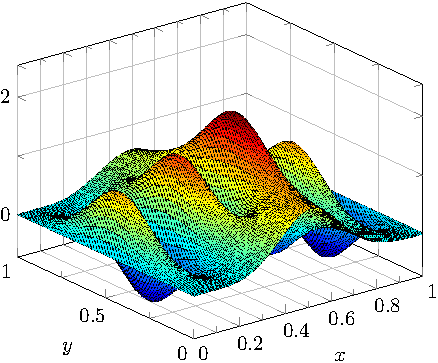
\includegraphics[width=0.7\columnwidth]{figures/Example.pdf}
    	\caption{3D surface obtained from PGFPlots \cite{PFGPlots}.}
    	\label{fig:figure}
    \end{figure}

\section{Tables}
	
        \tabref{tab:table} shows an example table of some astronomical objects. 

        \begin{table}[H]
        	\caption{Astronomical Object Data}
        	\label{tab:table}
        	\begin{tabular}{
        		>{\raggedright\arraybackslash}p{0.25\columnwidth}
        		>{\raggedright\arraybackslash}p{0.29\columnwidth}
        		>{\raggedright\arraybackslash}p{0.31\columnwidth}
        	}
        	\toprule
        	\textbf{Object} & \textbf{Type} & \textbf{Distance (Light Years)} \\
        	\midrule
        	Alpha Centauri & Star system & 4.37 \\
        	Betelgeuse & Red supergiant star & 642.5 \\
        	Andromeda & Spiral galaxy & 2.537 million \\
        	Earth & Planet & 0 \\
        	Sirius & Binary star system & 8.6 \\
        	\bottomrule
        	\end{tabular}
        	\tabletext{Note: The table contains data of some famous celestial objects.}
        \end{table}

        The \inlinecode{\tabletext{}} command is used to add notes to tables easily. 

\section{Document Data}

    \subsection{Front-Matter Footer Block*}

        A new block called \inlinecode{\docinfo{}}, has been added to the bottom right of the first page, acting as a floating element which stays fixed in place. This replaces the corresponding author block previously located above the abstract in earlier versions.

        The \inlinecode{\docinfo{}} block was created to give you greater control over supplementary document data, such as publication dates, licensing information, extended author details, and other front-matter notes. You can fully customize its content to suit your needs.

        Additionally, the new \inlinecode{\corres{}} command serves as a flexible alternative to \inlinecode{\thanks{}}. Since modifying the standard \inlinecode{\thanks{}} command can be complex and its positioning is often rigid, \inlinecode{\corres{}} was introduced to offer a more adaptable solution without sacrificing functionality. 
        
        \begin{note}
            You can use \verb|\corres{}| as many times as needed since it automatically ensures that each entry remains correctly associated. For best results, I recommend using text symbols rather than mathematical ones (e.g., \verb|\textasteriskcentered|, \verb|\textdagger|, etc.). 
        \end{note}

        If \inlinecode{\corres{}} is not used, \inlinecode{\docinfo{}} will automatically adjust its position. The implementation was designed to handle any combination of front-matter elements you might need when starting your document. In this example template, you’ll find a minimal demonstration that combines both to illustrate their interaction.

    \subsection{Headers and Footers*}

        \subsubsection{Headers}

            On all pages except the first, the document title and journal appear in the header. Since twoside layout is enabled, its position alternates depending on whether the page is odd or even.

        \subsubsection{Footers}

            In the first page, six elements display supplementary information for your document:

            \begin{itemize}
                \item \inlinecode{\journalname{}} — Displays the journal name, university, institute, company, or any institutional affiliation.
                \item \inlinecode{\theday{}} — Displays the current date.
                \item \inlinecode{\vol{}} — Specifies the volume number of the publication.
                \item \inlinecode{\no{}} — Specifies the issue number within the volume.
                \item \inlinecode{\journal{}} — Defines the full journal title.
                \item \inlinecode{\thepage} — Shows the current page number and the total count.
            \end{itemize}

             In all cases, you can freely rearrange or customize the order of these elements by modifying the class file to suit your needs. If any of them are not required, simply omit the corresponding command — the remaining elements will automatically adjust their spacing to remain evenly distributed.

\section{Rho Custom Packages}

    \subsection{Rhobabel.sty}
		
		This package have all the commands that automatically translate from English to Spanish when this custom package is defined. 
		
		By default, this document has its content in English. However, at the beginning of the document you will find a recommendation when writing in Spanish. 
		
		You may modify this package if you want to use other language than English or Spanish. This will make easier to translate your document without having to modify the class document.

    \subsection{Rhoenvs.sty}

        This package provides custom environments designed to enhance the visual presentation and structure of your document. Key examples include rhoenv, info, and note.
        
		Their style is defined by \inlinecode{rhoenvstyle} — allowing you to customize their appearance according to your document’s requirements.

		An example using the \inlinecode{rhoenv} environment is shown below.
		
		\begin{rhoenv}[frametitle=Custom Title]
			This is an example of the custom title environment. To add a title type this command \verb|[frametitle=Custom Title]| next to the beginning of this environment (as shown in this example).
		\end{rhoenv}

        The \inlinecode{info} and \inlinecode{note} are environments which have a predefined title and translate their title to Spanish automatically when this language is defined.

\section{Equations}

	\equref{eq:equation} shows the Schrödinger equation as an example. 

    \begin{equation}\label{eq:equation}
        i\hbar \frac{\partial }{\partial t}\Psi(\mathbf{r},t) = \left[\frac{-\hbar^2}{2m}\nabla^2 + V(\mathbf{r},t) \right]\Psi(\mathbf{r},t)
    \end{equation}
	
	The \inlinecode{amssymb} and \inlinecode{amsmath} packages were not required, as \href{https://ctan.org/pkg/stix2-otf/}{STIX2} font incorporates mathematical symbols for writing quality equations.
	
	\begin{note}
		If you would like to change the values that adjust the spacing above and below the equations, change the \verb|\eqskip| value until the preferred spacing is set. The default value is set to 9pt.
	\end{note}

\section{Codes}

	\subsection{Coding with Minted*}
	
		The \inlinecode{minted} package offers customized features for adding codes. In addition, the template is designed to work seamlessly with Fira Code, a monospaced font specially crafted for programming environments.

        If your are using a desktop app as \href{https://www.texstudio.org/}{TeXstudio}, try these steps to make this package work on Windows:
		
		\begin{enumerate}
			\item Install Python — A stable version (e.g., v.3.11)
			\item Open the terminal and type \inlinecode{pip install Pygments}.
			\item Update if a newer version is available.
			\item Go to TeXStudio settings and change the default compiler to \inlinecode{pdflatex --shell-escape -interaction=nonstopmode \%.tex}.
			\item Compile and wait for the result.
		\end{enumerate}
        
		\vspace*{-9pt}
        
		\begin{rhoenv}[frametitle=Caution]
			Ensure that \textbf{pygments} is properly installed and added to your system’s PATH. Otherwise, you may encounter compilation errors. Additionally, enable shell escape when compiling, as it is required for minted to process and highlight code.
		\end{rhoenv}
		
		In \href{https://es.overleaf.com/}{Overleaf}, this package is easier to use since it does not require any additional installations or modifications — just add the code as shown in the example. \coderef{lst:example} shows a Python example.
		
		\begin{code}
			\inputminted{python}{example.py}
            \caption{Python code example with minted.}
			\label{lst:example}
		\end{code}
		
		You can customize its design changing \inlinecode{\usemintedstyle} command. The different styles offered by the \href{https://ctan.org/pkg/minted}{minted package} can be preview through this link — \url{https://pygments.org/styles/}.

    \subsection{Coding with Listings}
	
		Since \inlinecode{minted} requires additional installations and can be complex in some desktop \TeX\ editors, you can use the \inlinecode{listings} package instead, which provides a simpler way to include code.
		
		\begin{code}
			\lstinputlisting[language=python]{example.py}
			\label{lst:example2}
            \caption{Python code example with listings.}
		\end{code}
		
		While \inlinecode{listings} is a simpler and widely supported package for code formatting, \inlinecode{minted} offers a more modern and powerful approach. It leverages the Pygments syntax highlighter to deliver superior coloring, language support, and styling options. One of its key advantages is the ability to easily switch between built-in color styles.
		
		In contrast, \inlinecode{listings} requires manual setup for colors, fonts, and formatting rules.
		For users who prefer fine-tuned customization, the styling options for \inlinecode{listings} are organized in \inlinecode{rho.cls} file and can be modified at any time to suit individual preferences.

	\subsection{Inline Code*}
	
		As shown in this template, inline code has a custom style for improved visual appeal. To use it, simply add \inlinecode{\inlinecode{}} command and place your code inside the braces.

\section*{Numberless section}
\addcontentsline{toc}{section}{Numberless section}

    Declaring a numberless section automatically inserts a square symbol before the title. This unique feature is specific to first-level sections within this class.
    
    As this symbol also affects the table of contents and references titles, users who prefer to disable it may edit the section styling parameters in \inlinecode{rho.cls}.

\section{Bibliography}
		
	Bibliography management is handled by \inlinecode{biblatex}, with the default citation and reference style set to IEEE. The \inlinecode{citestyle=numeric-comp} option is enabled, allowing multiple citations to be grouped within a single bracket (e.g., \cite{davis2023signalflow,bell2022codefont}). The citation format can be customized directly in \inlinecode{rho.cls} to suit any preferred style.

\section*{FAQ}
\addcontentsline{toc}{section}{FAQ}

    \subsection*{How do I manage my references?}
    \addcontentsline{toc}{subsection}{How do I manage my references?}
        
        To manage your references, I recommend using the tool \href{https://www.scribbr.es/citar/generador/folders/73QOXYsCwMRu4ifQaN65mx/lists/msTfx7GJjIAOUkufbISnA/}{scribbr}. You can simply enter the URL or create your own citation, and then export it to \LaTeX{} using the options in the three-dot menu.
            
        The generated citation can be copied and pasted into \inlinecode{rho.bib}, the file designated for bibliography management. You may rename this file, but if you do, remember to update the \inlinecode{\addbibresource} command in \inlinecode{rho.cls} under the biblatex section.
    
        \begin{note}
            Some platforms, such as Google Scholar or scientific journals, provide citations directly in BibTeX format. Therefore, check if there is a ``how to cite this document'' section to streamline the citation process even further.
        \end{note}

        If you have any further questions, you can refer to the following page — \href{https://es.overleaf.com/learn/latex/Bibliography_management_with_biblatex}{Bibliography management with biblatex}.
        
    \subsection*{What should I do with the example files?}
    \addcontentsline{toc}{subsection}{What should I do with the example files?}

        The template includes sample content — such as an example figure, bibliography entries, and the \inlinecode{example.py} script — to demonstrate how the layout and features work. Once you start customizing the document for your own use, feel free to delete all example files and entries you don’t need.

    \subsection*{How do I place equations easily?}
    \addcontentsline{toc}{subsection}{How do I place equations easily?}

        For equations, we have two options: inline or on its own line. For inline equations, simply place a dollar sign (\$) at the beginning and end of the equation. However, if you want the equation to be displayed on its own line, you need to use the equation environment.
        
        If you find it challenging to write formulas directly in \LaTeX, you can use text editors like Word. In the equations menu, you can select \LaTeX\ in the conversion section and copy and paste the equation you wrote into one of these two environments.

    \subsection*{How do I change the paper size?}
    \addcontentsline{toc}{subsection}{How do I change the paper size?}

        By default, this class was adapted for a4paper and test it with letterpaper. The following paper sizes are available in \LaTeX:

        \begin{itemize}
            \item letterpaper (11 $\times$ 8.5 in)
            \item legalpaper (14 $\times$ 8.5 in)
            \item executivepaper (10.5 $\times$ 7.25 in)
            \item a4paper (21 $\times$ 29.7 cm)
            \item a5paper (21 $\times$ 14.8 cm)
            \item b5paper (25 $\times$ 17.6 cm)
       \end{itemize}

\section*{Contact me}
\addcontentsline{toc}{section}{Contact me}
    
    Have questions, suggestions, or an idea for a new feature? Found a bug or working on a project you’d like to invite me to?  
    
    Feel free to reach out — I’d be happy to help, collaborate, or fix the issue.  Your feedback helps me improve my templates!

    \AtBeginEnvironment{tabular}{\normalsize\sffamily\selectfont}
    \begin{center}
        \setlength{\tabcolsep}{3pt}
        \begin{tabular}{cl}
            \faEnvelope & \href{mailto:memo.notess1@gmail.com}{memo.notess1@gmail.com} \\
            \faGlobe{} & \href{https://memonotess1.wixsite.com/memonotess}{memonotess.com} \\
            \faInstagram{} & \href{https://www.instagram.com/memo.notess/}{@memo.notess}
        \end{tabular}
    \end{center}

\section*{Github Repository}
\addcontentsline{toc}{section}{Github Repository}

    Visit the repository to access the source code, track ongoing development, report issues, and stay up to date with the latest changes.

    \begin{center}
        \setlength{\tabcolsep}{3pt}
        \begin{tabular}{cl}
             \faGithub &  \url{https://github.com/MemoJimenez/Rho-class}\\
        \end{tabular}
    \end{center}

\section*{Supporting}
\addcontentsline{toc}{section}{Supporting}

    Enjoyed this document class? Check out tau-class, my very first \LaTeX{} template.

    \begin{center}
        \setlength{\tabcolsep}{3pt}
        \begin{tabular}{cl}
             \faLink &  \href{https://es.overleaf.com/latex/templates/tau-class-lab-report-template/chhshmhxstsq}{https://es.overleaf.com/latex/templates/tau-class}\\
        \end{tabular}
    \end{center}
    
    \subsection*{Any contributions are welcome!}
    \addcontentsline{toc}{subsection}{Any contributions are welcome!}
    
        Coffee keeps me awake and helps me create better \LaTeX\ templates. If you wish to support my work, you can do so through PayPal: 

        \begin{center}
            \setlength{\tabcolsep}{3pt}
            \begin{tabular}{cl}
                 \faPaypal & \textbf{\url{https://www.paypal.me/GuillermoJimeenez}}\\
            \end{tabular}
            \vskip9pt
            Enjoy writing with rho-class!
        \end{center}

\end{document}